\documentclass[12pt,oneside,french]{article}
\usepackage{mathptmx}
\usepackage{helvet}
\usepackage{courier}
\usepackage[T1]{fontenc}
\usepackage[utf8]{inputenc}
\setcounter{secnumdepth}{3}
\setcounter{tocdepth}{3}
\usepackage{babel}
\addto\extrasfrench{%
   \providecommand{\og}{\leavevmode\flqq~}%
   \providecommand{\fg}{\ifdim\lastskip>\z@\unskip\fi~\frqq}%
}

\usepackage{amsmath}
\usepackage{amssymb}
\usepackage[unicode=true,pdfusetitle,
 bookmarks=true,bookmarksnumbered=false,bookmarksopen=false,
 breaklinks=false,pdfborder={0 0 1},backref=section,colorlinks=false]
 {hyperref}

\makeatletter
\usepackage{graphicx}
\usepackage{babel}
%
\usepackage{fancyhdr}
\pagestyle{fancy}
\rfoot{}
\chead{}
\cfoot{}
\lhead{
 \textit{22\textsuperscript{ème} Congrès Français de Mécanique}}              
\rhead{
 \textit{Lyon, 24 au 28 Août 2015}}

\begin{document}

\vspace{25pt}
\begin{center}
\baselineskip=13pt
{\huge{}\textbf{Retour d'expériences sur l'utilisation de plateformes Web$^{2.0}$ "Webwork" et "Ipython Notebook" }}

\vspace{13pt}
{\large{}\textbf{Marc BUFFAT}}{\large{}\textsuperscript{\textbf{a}}}

\vspace{13pt}
(a) département de mécanique, université Claude Bernard Lyon 1, \\ \it{marc.buffat@univ-lyon1.fr}
\end{center}

\vspace{13pt}
\baselineskip=13pt
\leftskip=0pt
{\Large{}\textbf{Résumé : }}
\vspace{13pt}

\textit{
	Une grande majorité d'étudiants en Licence et Master de mécanique ont
	des lacunes  dans le domaine de la maîtrise de l’outil mathématique et
	de la programmation scientifique. Par manque d'autonomie et de méthodes
	de travail, ces étudiants ne font pas d'eux même régulièrement les
	exercices de mathématiques ou de programmation nécessaires pour acquérir
	cette maîtrise. C'est pour aider ces étudiants que depuis plusieurs
	années nous expérimentons au département de mécanique de l'université
	Lyon 1 de nouveaux outils pédagogiques.  Durant cet exposé je
	présenterai un retour d'expérience sur l'utilisation de Webwork, un
	système de devoirs en ligne auto corrigés, et de IPython notebook, une
	interface web enrichie mixant l'exécution de code Python, du texte avec
	une notation $\LaTeX$, des tracés graphiques et de la vidéo.
}


\vspace{13pt}
{\Large{}\textbf{Abstract : }}
\vspace{13pt}

\textit{
A  majority of students in the mechanical engeneering department at the
university do not adequately master mathematical tool and scientific
programming.  To help the students to master these tools, we experience since
several years at the mechanical engeneering department of the University Lyon 1
new teaching tools.  During this presentation I will present feedback on the
use of WebWork, a web-based interactive system designed to make homework in
mathematics and the sciences more effective and efficient, and the IPython
notebook, a web-based interactive computational environment, in which you can combine code execution,
rich text, mathematics, plots and rich media.
}


\vspace{27pt}
{\large{}\textbf{Mots clefs : Devoirs en ligne, WebWork, IPython, MOOC}}

\vspace{13pt}
{\Large{}\textbf{1 Introduction}}
\vspace{13pt}

La filière mécanique à l'université étant par nature non sélective, le public
d'étudiants en Licence et Master de mécanique est extrêmement varié, en
particulier en terme de formation initiale. Pour une majorité d'étudiants, on
constate ainsi des lacunes importantes dans le domaine de la maîtrise de
l'outil mathématique et de la programmation scientifique.  Or cette maîtrise,
indispensable pour des études en mécanique,  passe par une mise en pratique
régulière de résolution d'exercices de mathématiques et d'écriture de
programmes. Par manque d'autonomie et de méthodes de travail, beaucoup
d'étudiants ne parviennent cependant pas par eux mêmes à s'astreindre à faire ces
exercices en utilisant par exemple les livres d'exercices disponibles dans les bibliothèques
universitaires.

C'est ainsi, que depuis plusieurs années, les enseignants du département de
mécanique de l'université Claude Bernard Lyon 1 expérimentent des pratiques
pédagogiques nouvelles et en particulier l'utilisation d'outils TICE pour aider
à la réussite de ces étudiants \cite{buffat1,buffat2,buffat3}. 

Lors de cette présentation, je donnerai un retour d'expérience sur la mise en place
et l'utilisation de ces pratiques pédagogiques au sein du département de mécanique de l'UCB Lyon 1.

\vspace{13pt}
{\Large{}\textbf{2 Mise en place}}
\vspace{13pt}

L'approche utilisée se veut pragmatique, en essayant d'améliorer ce qui existe dans le
contexte d'un enseignement en présentiel et en tenant compte des moyens
"limités" de l'université. Au département de mécanique, nous avons choisi 
de privilégier l'utilisation de logiciels libres, plutôt que des alternatives commerciales
 comme Maple T.A. et Matlab.
\begin{figure}
	\begin{center}
		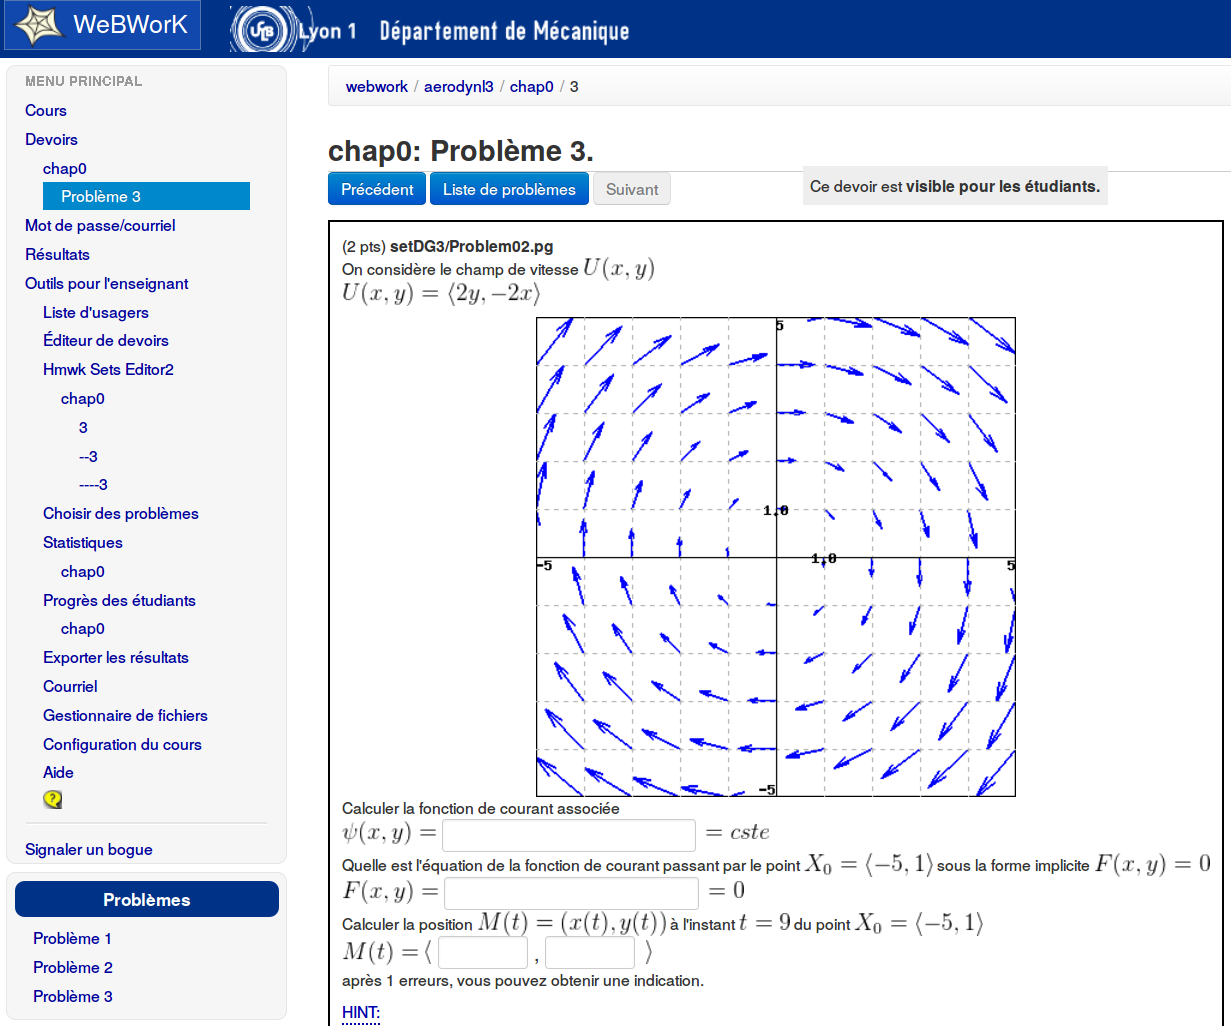
\includegraphics[width=0.4\paperwidth]{webwork1.png}
	\end{center}
	\caption{Exemple d'exercice WebWork en mécanique des fluides}\label{fig1}
\end{figure}

D'un point de vue technique, cela nous a conduit à
installer et gérer au sein du département de mécanique notre propre portail pédagogique
(\href{http://ufrmeca.univ-lyon1.fr/moodle}{http://ufrmeca.univ-lyon1.fr/moodle}),
basé sur le LMS Moodle, qui assure une très forte interopérabilité avec
différentes plateformes numériques d'apprentissage utilisées tels que 
Webwork\cite{webwork}, Sage, SageCell\cite{sage} et Ipython
Notebook\cite{ipython}. Un appel à projet TICE a permis de financer les serveurs informatiques où sont
installés ces outils dans  des machines virtuelles, facilement administrables sous Linux.

La plateforme Webwork\cite{webwork} est un logiciel libre qui permet aux
étudiants de faire des devoirs de mathématiques et de sciences en ligne
en utilisant un simple navigateur.
WeBWorK est développé depuis 2001 par le département de mathématique de
l'université de Rochester et est soutenu par la MAA (Mathematical Association
of America) et la NSF (National Science Foundation). Il contient une
bibliothèque de plus de 20000 exercices  sur  l'algèbre, les mathématiques
discrètes, les probabilités et statistiques, le calcul simple et multivariée,
les équations différentielles, l'algèbre linéaire et l'analyse complexe.
Utilisée dans les cours de mathématiques, de mécanique des fluides et des
solides, de calcul scientifique en Licence, et dans les cours de mise à niveau,
d'éléments finis, de méthodes numériques et EDP en Master, WebWork permet de
donner des devoirs personnalisés aux étudiants (chaque étudiant a un exercice
avec des paramètres différents) avec auto correction et auto-évaluation (voir figure \ref{fig1}). 

Le second outil utilisé est le notebook Ipython\cite{ipython} qui
permet une interactivité plus grande durant les séances de cours en intégrant
dans une interface Web l'exposition des principes (avec l'utilisation de $\LaTeX$ ), la simulation
informatique (avec Python), voire d’accéder à des ressources en ligne (pages
wikipedia, video youtube, ...) (voir figure \ref{fig2}).
\begin{figure}
	\begin{center}
		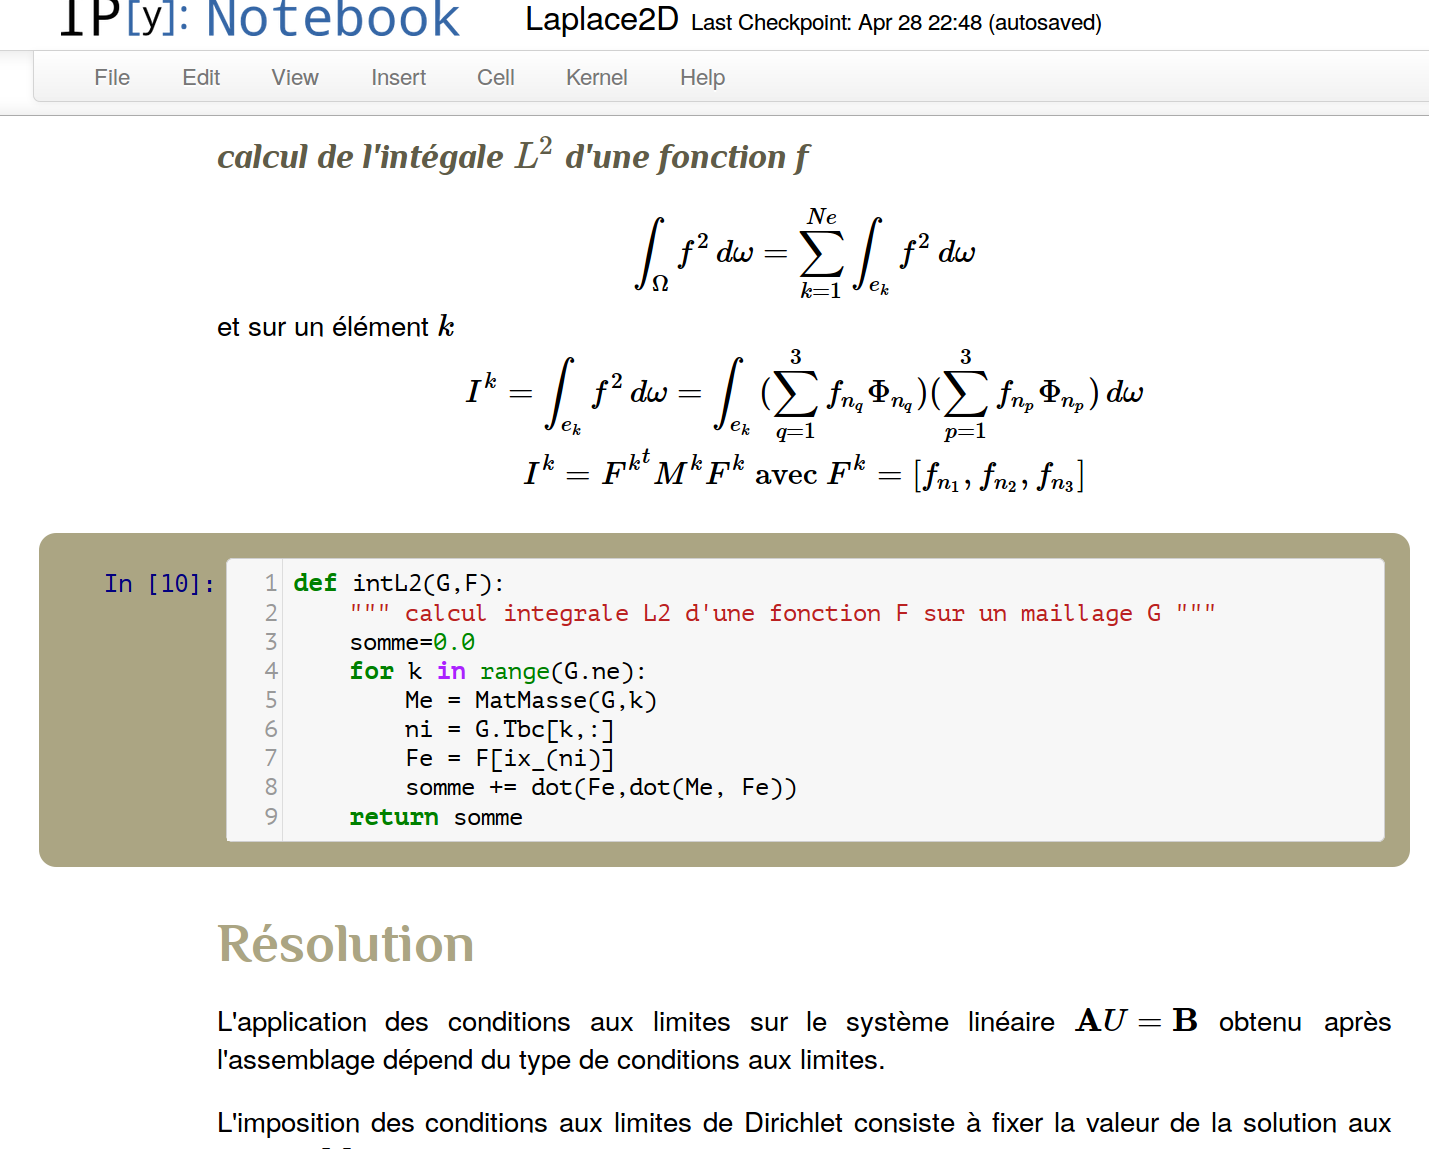
\includegraphics[width=0.3\paperwidth]{ipython1.png}\hspace{0.4cm}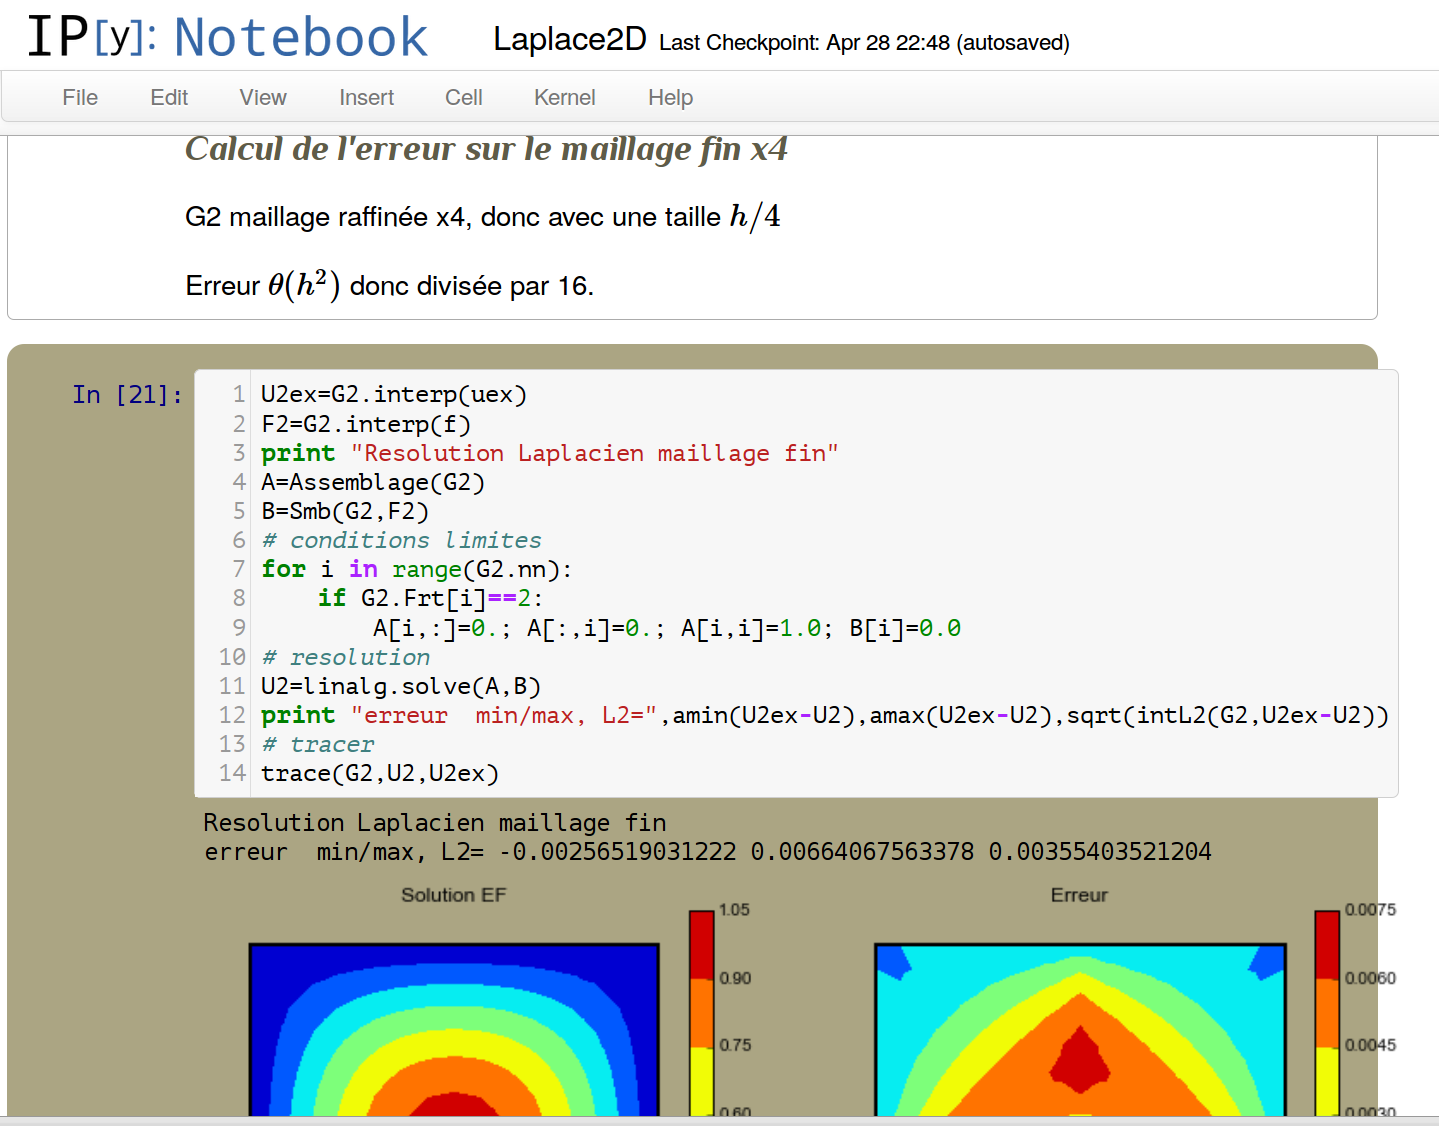
\includegraphics[width=0.3\paperwidth]{ipython2.png}
	\end{center}
	\caption{Exemple de cours avec le NoteBook Ipython }\label{fig2}
\end{figure}


\vspace{13pt}
{\Large{}\textbf{3 Bilan et perspective}}
\vspace{13pt}

Lors de l’exposé je présenterai ces deux outils Webwork et Ipython notebook, le retour
d’expérience de leur utilisation, les difficultés rencontrées, ainsi que le projet de MOOC
INPROS\cite{inpros} "Introduction à la Programmation Scientifique" dont 
l’objectif est l’apprentissage d’une méthodologie de programmation scientifique,
axé sur la pratique de la programmation (en Python) et des exercices en ligne
utilisant les outils SageCell et Webwork, à travers un simple navigateur sur PC
portable ou tablette.

%il est fortement recommandé d'utiliser l'environnement thebibliography
%\begin{thebibliography}{9}
%  \bibitem{lamport94}
%       Leslie Lamport,
%     \emph{\LaTeX: A Document Preparation System}.
%  Addison Wesley, Massachusetts,
%2nd Edition,
%1994.
%\end{thebibliography}
\bibliographystyle{plain}
\begin{thebibliography}{99}

	\bibitem{buffat1} {\sc M. Buffat, A. Mille and M. Picasso},{\sl
		"Feedbacks on MOOCS"}, { congrès d'analyse numérique CANUM
		2014, ESAIM: proceedings and surveys, March 2015, Vol. 49, p.
	66-80}.

	\bibitem{buffat2} {\sc M. Buffat},{\sl "Ipython Notebook pour
		l'enseignement"},{ conférence Python: PyconFR 2014, 25-28
		octobre, Lyon 2014}.

	\bibitem{buffat3} {\sc M. Buffat},{\sl "WebWork un système de devoirs
		en ligne sous Moodle"},{ conférence MoodleMoot2009, INSA de
		Lyon Juillet 2009}.

	\bibitem{inpros} {\sc INPROS}, {\sl "Introduction \`a la Programmation
		Scientifique"},\href{http://inpros.univ-lyon1.fr}{inpros.univ-lyon1.fr}.

	\bibitem{ipython} {\sc IPython},{"Python Interactive
		computing"},\href{http://www.ipython.org}{www.ipython.org}.

	\bibitem{sage} {\sc SAGE}, {\sl "logiciel libre de math\'ematiques en
		ligne"},\href{http://www.sagemath.org}{www.sagemath.org}.

	\bibitem{webwork} {\sc WEBWORK}, {\sl "syst\`eme de devoirs de
		math\'ematique en ligne"},\href{http://webwork.maa.org}{webwork.maa.org}.

% NE PAS MODIFIER LA LIGNE SUIVANTE
\end{thebibliography}
\end{document}
%
